\section{Major update to OpenMC Heat Source} 
\label{s:openmc_tallies}

In addition to the changes in NekRS some major changes were introduced in the way Cardinal interfaces with OpenMC.

To capture heat generation in the OpenMC simulation, a tally scoring the amount of total recoverable fission energy per source particle is applied to the outer cell of each pebble in the bed. 
These tallies are created at runtime during the problem setup by using a list of pebble centers to locate the uppermost cell in the CSG geometry hierarchy containing that point.

As summarized in \autoref{eq:heat_source_normalization}, the energy deposition for each pebble, $\hat{q}_{i}$, is normalized by the total energy deposition in the bed and multiplied by the the total thermal power of the reactor, $Q$ to obtain a an average heat generation rate for each pebble, $q_i$. This value is then divided by the volume of each pebble, $V_p$, to obtain a volumetric heat generation rate, $q'''_i$.

\begin{equation}
    \label{eq:heat_source_normalization}
    q'''_i = \frac{Q q_i}{V_{p}\sum_{i}{\hat{q_i}}} = \frac{[W][J/source]}{[cm^{3}] [J/source]} = \frac{[W]}{[cm^{3}]}
\end{equation}

This results in a single average heating value for the entire pebble. Before being transferred to the MOOSE mesh, these values are normalized by the total heat

For improved spatial resolution of heat generation in the pebble bed, unstructured mesh tallies have been implemented in OpenMC.
\autoref{fig:pebble_umesh} provides an example of this capability applied to a single pebble.
The unstructured mesh representation relies on a LibMesh mesh instance and currently conforms to the OpenMC model in which the mesh structure and tally data are separated.
The separation of this information allows the unstructured mesh to be applied in a mesh filter without knowledge of the underlying mesh type.
The mesh filter can then be used in one or more tallies in combination with other specified filters, scores, and nuclides to form a tally.
Calls into the LibMesh library from OpenMC are agnostic to the type of elements being used, so meshes can be formed using any element type supported by LibMesh.

\begin{figure}
    \centering
    \raisebox{-0.5\height}{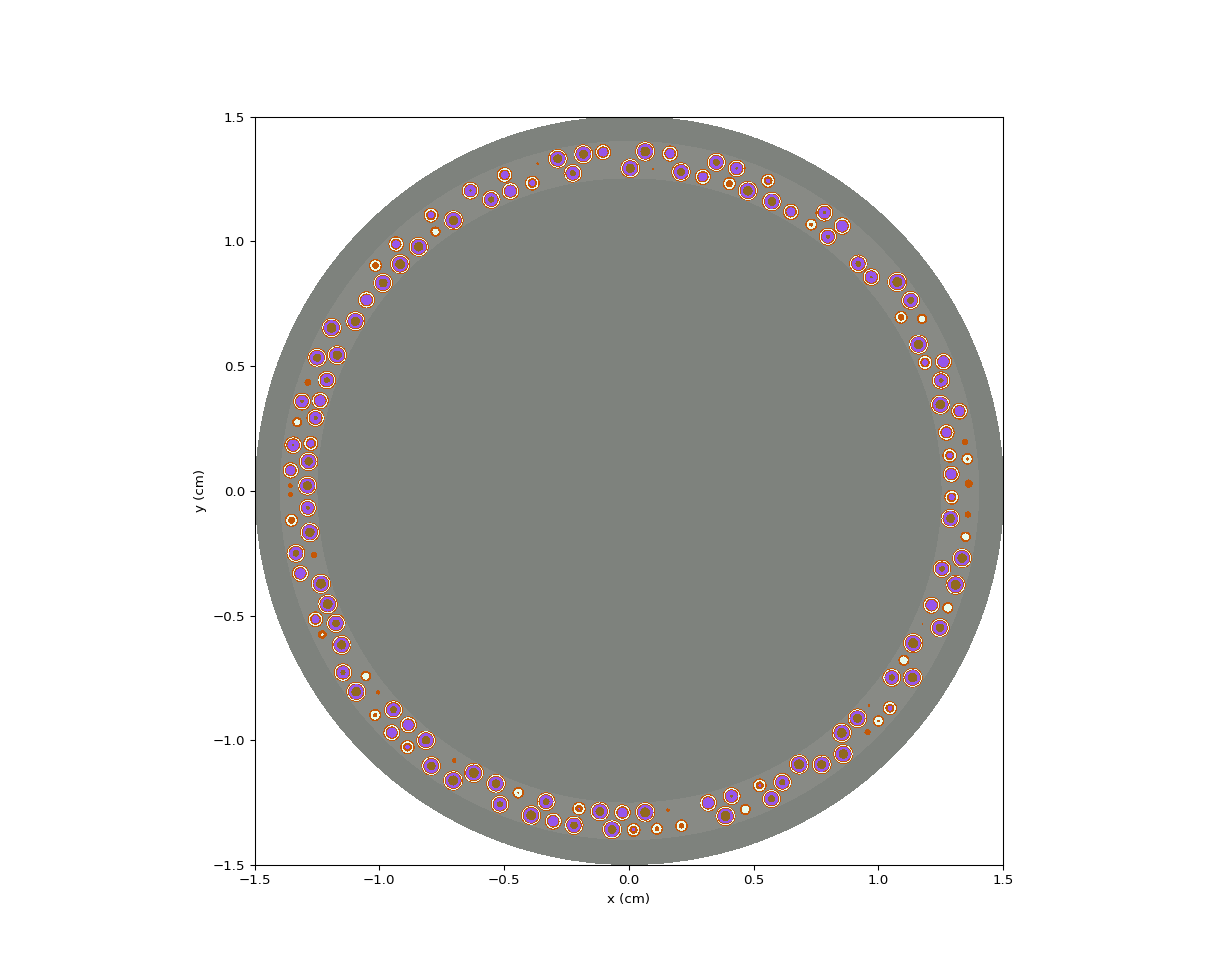
\includegraphics[width=0.5\textwidth]{Figures/pebble_cutaway}}
    \hspace*{.2in}
    \raisebox{-0.5\height}{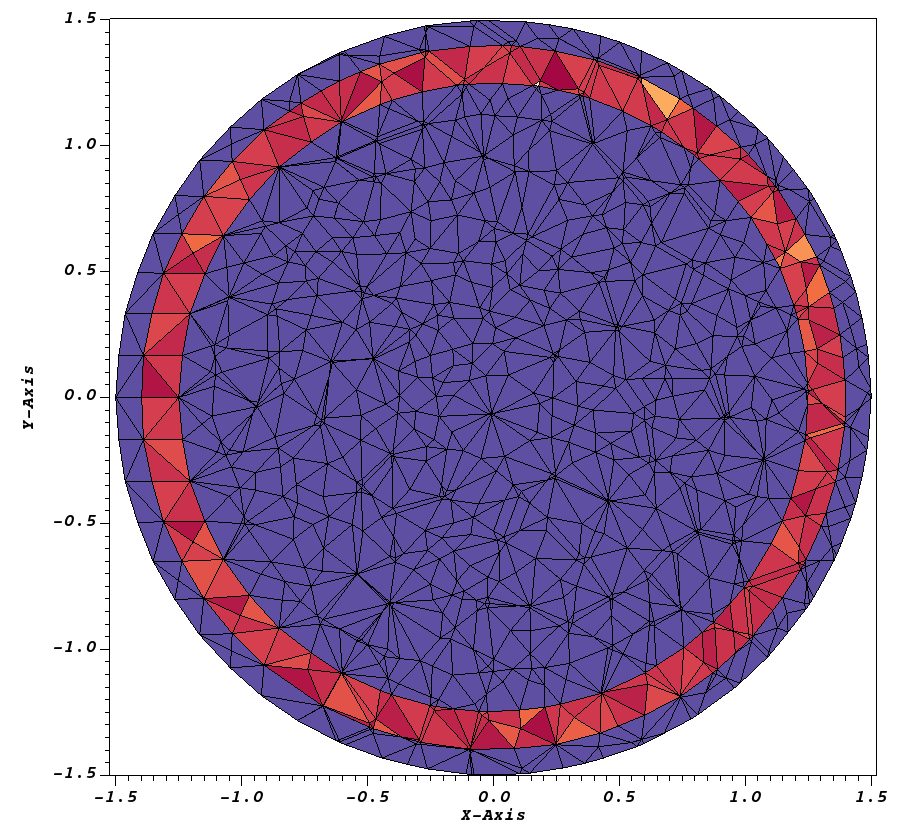
\includegraphics[width=0.365\textwidth]{Figures/umesh_ex}}
    \caption{Qualitative view of a heating tally on an unstructured mesh. Left: Cut-away of the pebble geometry as represented in OpenMC. Right: Result of an applied heating tally where heating only occurs in the region of the pebble containing TRISO particles.}
    \label{fig:pebble_umesh}
\end{figure}

A mesh for each pebble is applied in the Cardinal problem to capture the heat generation distribution throughout the pebble bed.
To avoid replicating a mesh representing all of the pebbles from either MOOSE or NEKRS, an option for adding translations to mesh filters was introduced in OpenMC.
Placing the translation at this layer of the tally structure allows all tallies to rely on a single LibMesh mesh instance acting as a template for a single pebble as shown in \autoref{fig:umesh_tally_steup}.
This results in a very low memory footprint for the tally, even when extended to an entire pebble bed.

\begin{figure}[ht]
    \centering
    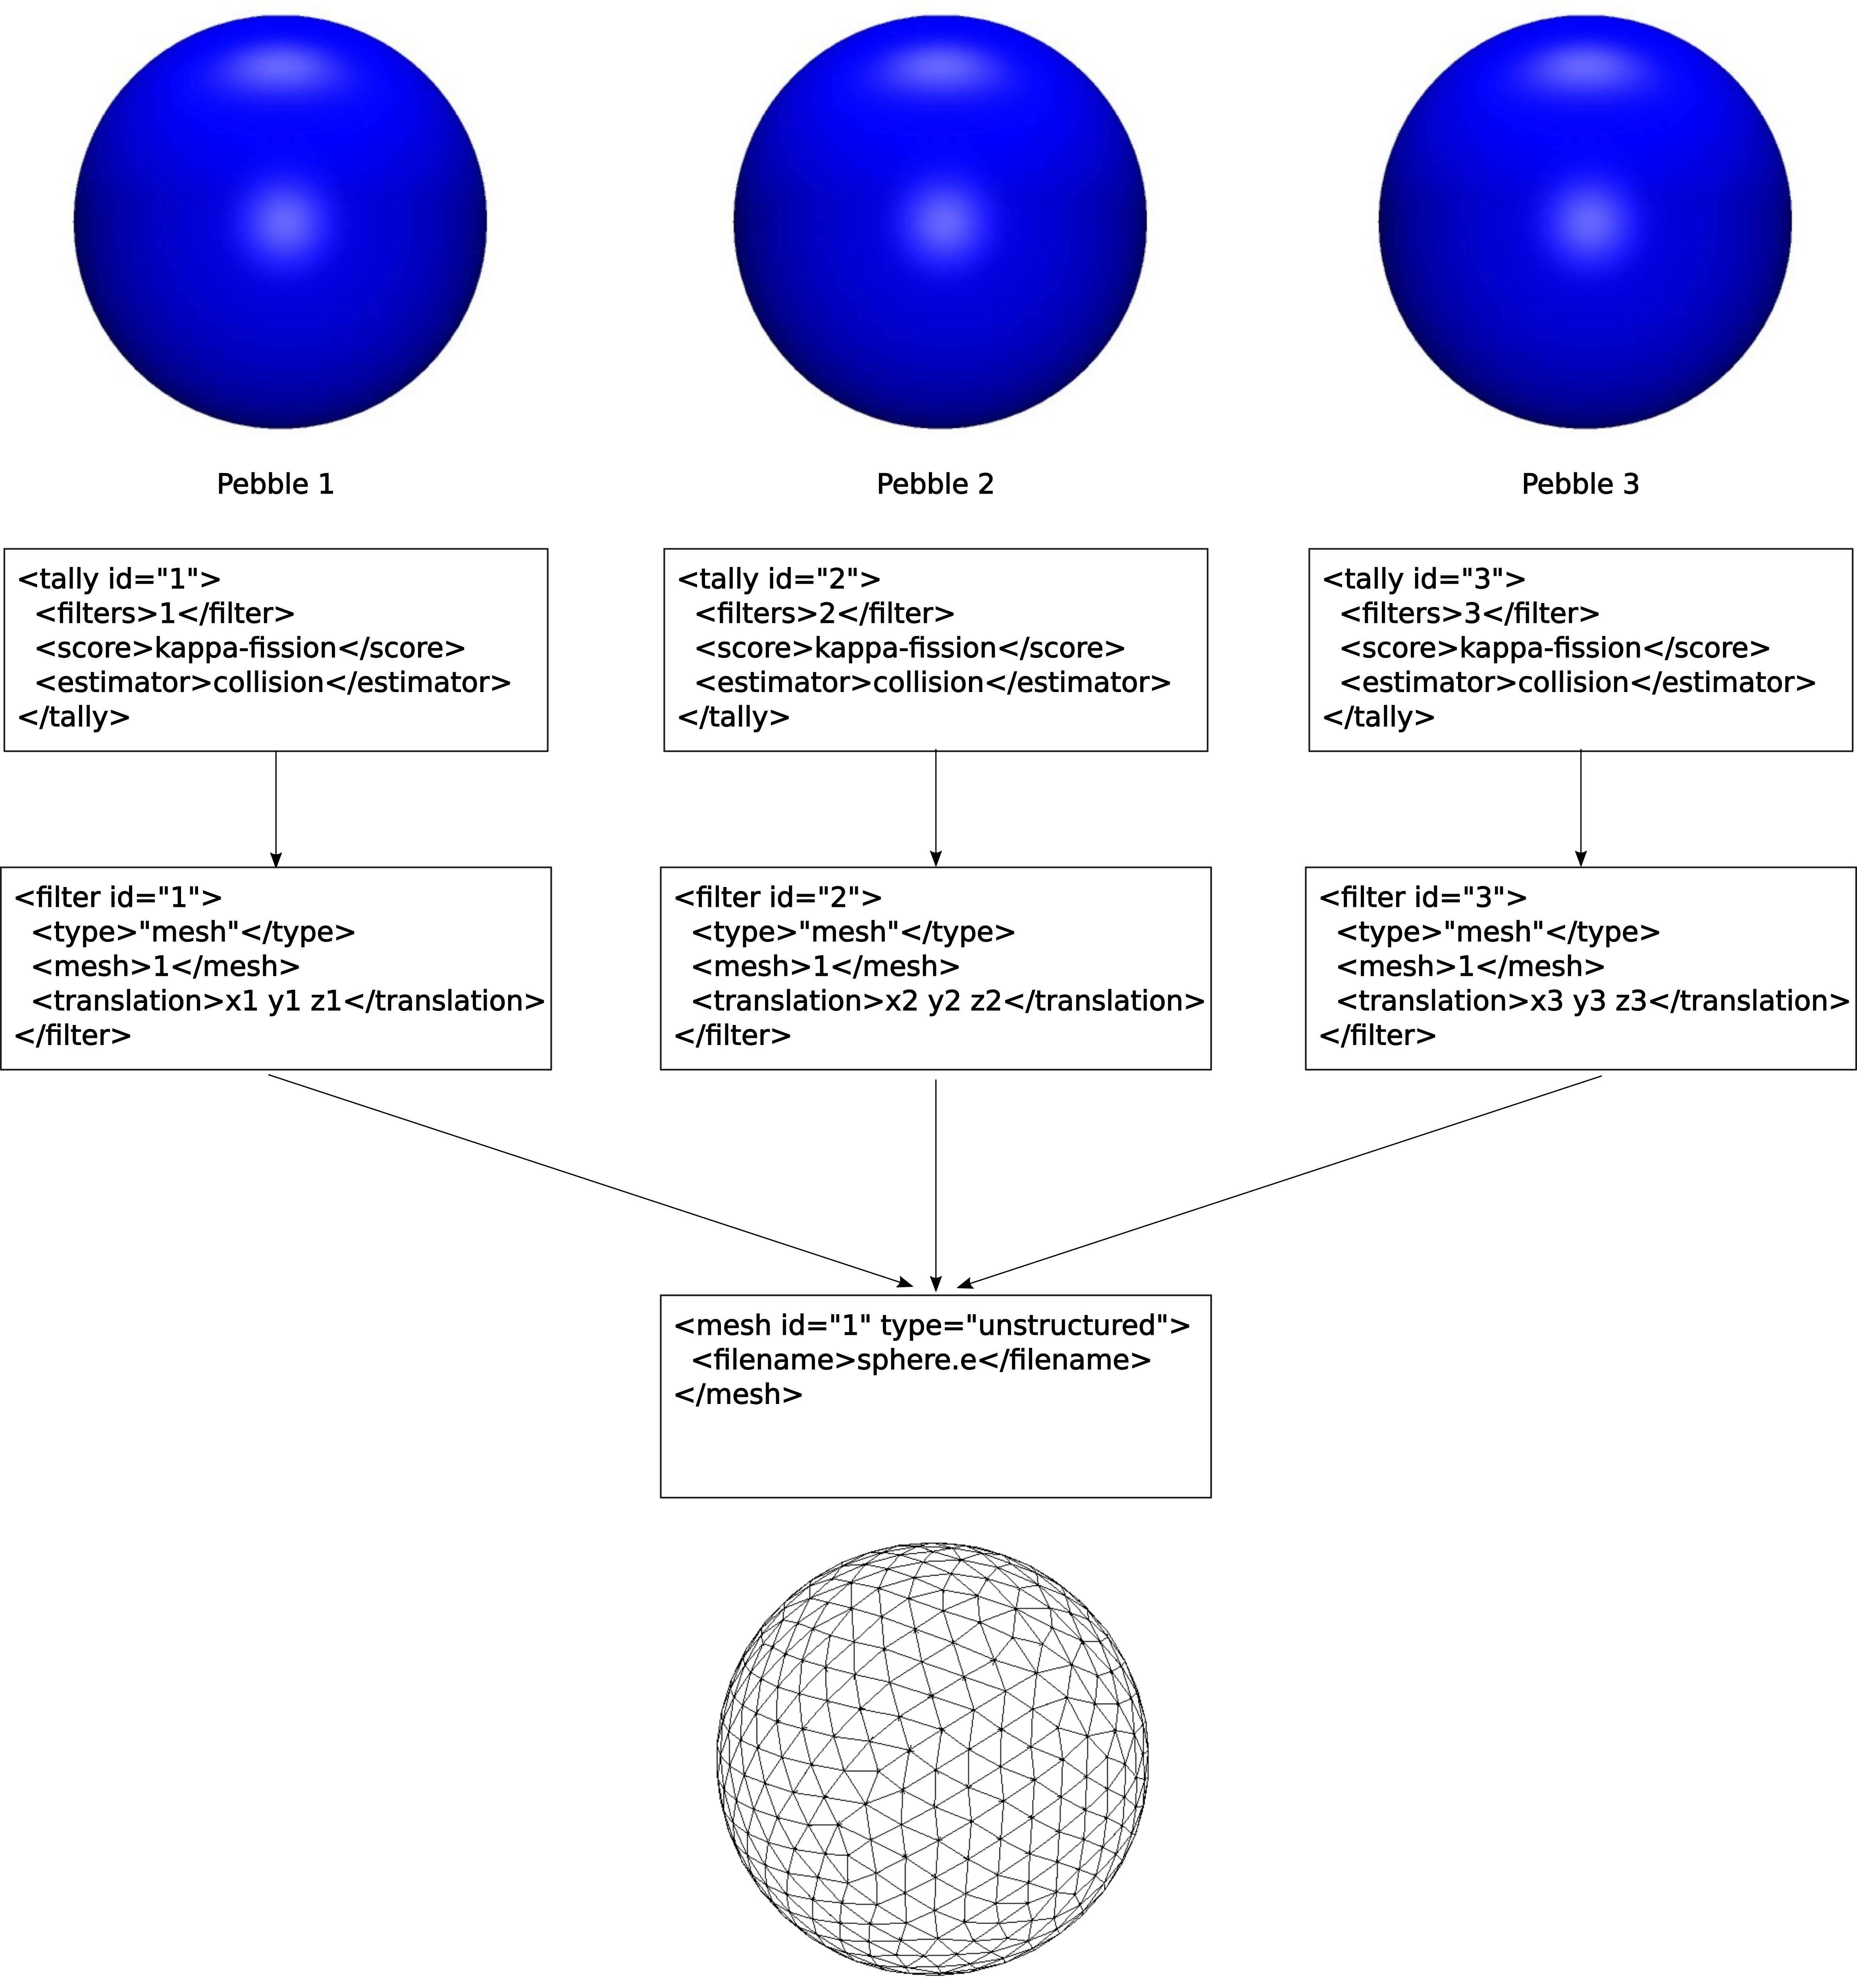
\includegraphics[width=\textwidth]{Figures/umesh_tally_diagram}
    \caption{Organization of unstructured mesh tallies for heat generation in OpenMC.}
    \label{fig:umesh_tally_steup}
\end{figure}

The translation values for each mesh filter are set using the list of pebble centers provided in the MOOSE input file.
During problem initialization, these translations are used to adjust the location of element centers in the mesh template when transferring heat generation value to MOOSE.
% Element volumes can be determined directly from the 
As the only additional input information required for the unstructured mesh tallies is the specification of a mesh template input file, the unstructured mesh tallies can be specified at runtime by setting the appropriate tally type parameter in the OpenMC MOOSE input file.

\subsection{Updating Temperature Values}

Temperature values from MOOSE are updated in OpenMC using an average temperature value at the pebble center.
To simplify the process of updating the temperature of all cells inside the pebble, an option has been added in OpenMC to propagate a temperature value into all cells filled by a material if the cell whose property is being updated contains a universe or lattice.
